\begin{frame}
    \frametitle{Syntaktische Analyse}
    \begin{itemize}
    \item Prüfung, ob Eingabeprogramm syntaktisch korrekt ist
    \item Verschiedene Arten von Parsern
    	\begin{itemize}
    	\item LL(1)- und (S)LL(k)-Parser
    	\item LR- und LALR-Parser
    	\end{itemize}
    \item MiniJava-Grammatik in SLL(3) umformbar \pause
    \begin{itemize}
    	\item Beispiel: \code{a[}
    	\item[] $\rightarrow$ Deklaration einer lokalen Variable: \code{a[] q;}
    	\item[] $\rightarrow$ Zugriff auf einen Array: \code{a[3] = 3;}
    \end{itemize} \pause
    \item mögliche Verfahren
	    \begin{itemize}
		\item Tabellenbasiert
		\item rekursiver Abstieg
		\only<4->{
            \begin{tikzpicture}[overlay]
                \node at (.8,.2) {
\includegraphics[angle=5,origin=c,width=1.5cm,keepaspectratio=true]{logos/mj++logo.png}};
            \end{tikzpicture}
        }
    	\end{itemize}
    \end{itemize}
\end{frame}

\begin{frame}
	\frametitle{AST-Aufbau}
	\begin{itemize}
	\item Quelltext muss in passenderes Format umgewandelt werden
	\item[] $\rightarrow$ Code-Hierarchie darstellen durch \textbf{abstrakten Syntaxbaum (AST)}
	\item Zeichen ohne Bedeutung werden nicht übernommen
	\item Aufbau während des Parsens
	\end{itemize}
\end{frame}

\begin{frame}
	\frametitle{Beispiel}
	\token{class}, \token{Foo}, \token{\{}, \token{public}, \token{int}, \token{bar}, \token{(}, \token{)}, \token{\{}, \ldots \\
        wird zu \\
     \begin{center}
     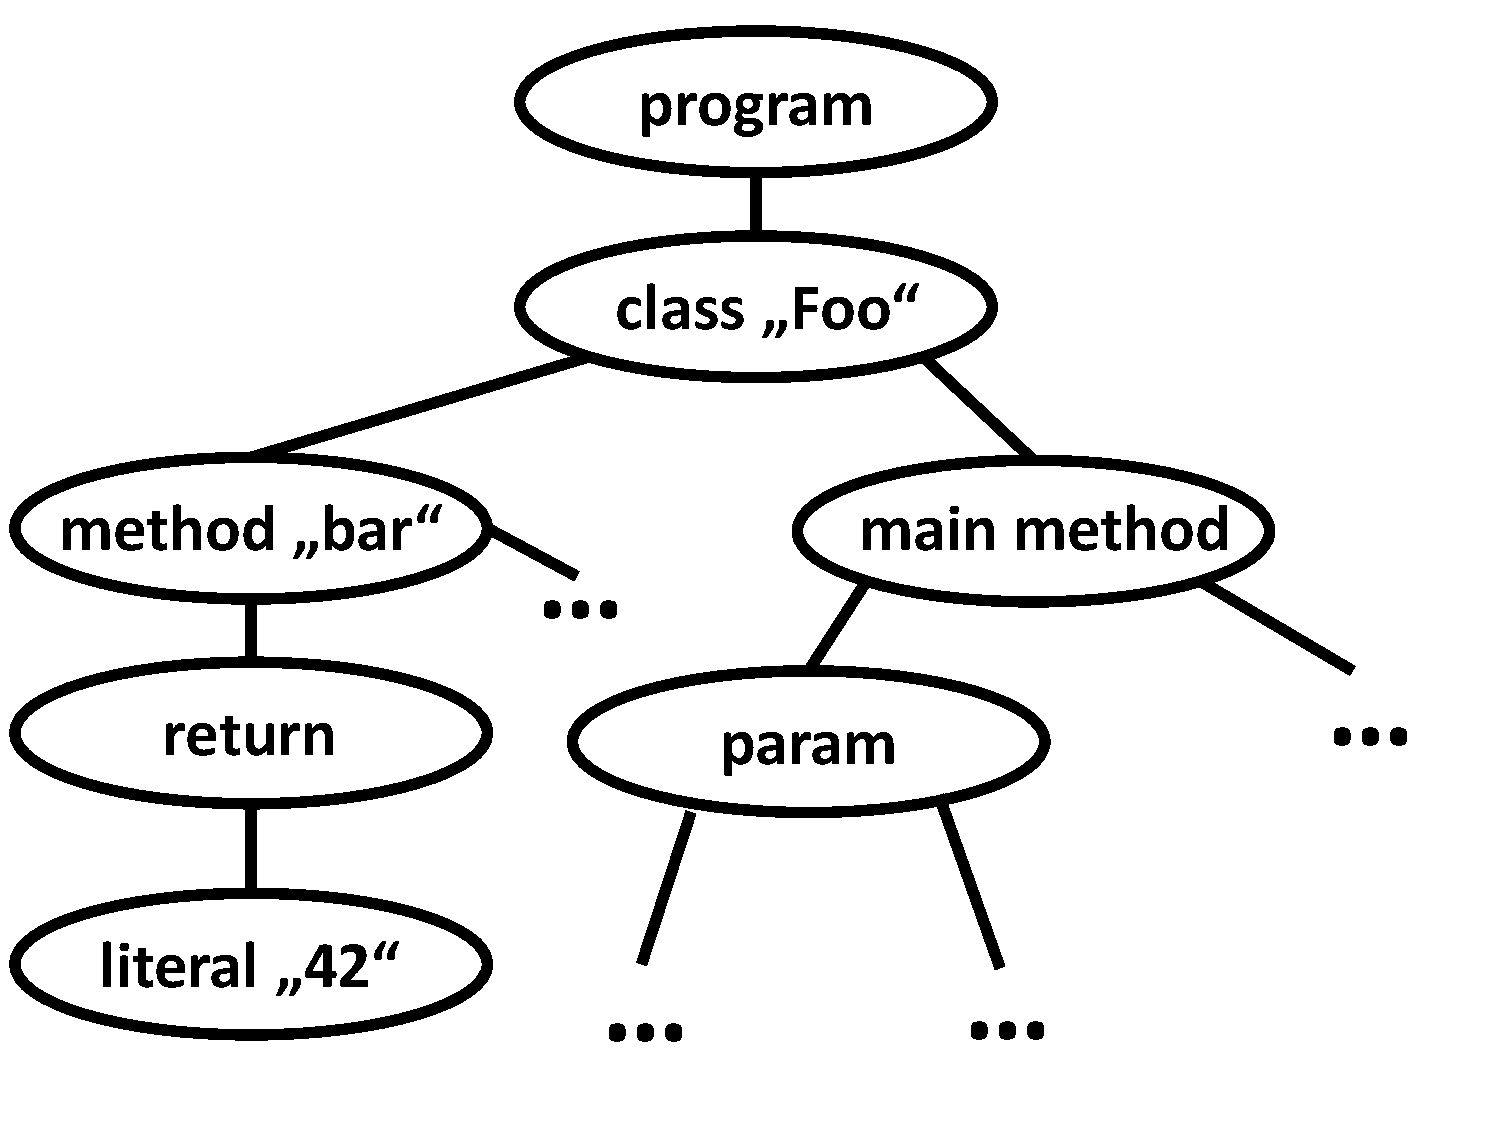
\includegraphics[scale=0.3]{images/AST.pdf}
     \end{center}
\end{frame}
